\documentclass[fleqn, 10pt]{beamer}\usepackage[]{graphicx}\usepackage[]{color}
% maxwidth is the original width if it is less than linewidth
% otherwise use linewidth (to make sure the graphics do not exceed the margin)
\makeatletter
\def\maxwidth{ %
  \ifdim\Gin@nat@width>\linewidth
    \linewidth
  \else
    \Gin@nat@width
  \fi
}
\makeatother

\definecolor{fgcolor}{rgb}{0.345, 0.345, 0.345}
\newcommand{\hlnum}[1]{\textcolor[rgb]{0.686,0.059,0.569}{#1}}%
\newcommand{\hlstr}[1]{\textcolor[rgb]{0.192,0.494,0.8}{#1}}%
\newcommand{\hlcom}[1]{\textcolor[rgb]{0.678,0.584,0.686}{\textit{#1}}}%
\newcommand{\hlopt}[1]{\textcolor[rgb]{0,0,0}{#1}}%
\newcommand{\hlstd}[1]{\textcolor[rgb]{0.345,0.345,0.345}{#1}}%
\newcommand{\hlkwa}[1]{\textcolor[rgb]{0.161,0.373,0.58}{\textbf{#1}}}%
\newcommand{\hlkwb}[1]{\textcolor[rgb]{0.69,0.353,0.396}{#1}}%
\newcommand{\hlkwc}[1]{\textcolor[rgb]{0.333,0.667,0.333}{#1}}%
\newcommand{\hlkwd}[1]{\textcolor[rgb]{0.737,0.353,0.396}{\textbf{#1}}}%
\let\hlipl\hlkwb

\usepackage{framed}
\makeatletter
\newenvironment{kframe}{%
 \def\at@end@of@kframe{}%
 \ifinner\ifhmode%
  \def\at@end@of@kframe{\end{minipage}}%
  \begin{minipage}{\columnwidth}%
 \fi\fi%
 \def\FrameCommand##1{\hskip\@totalleftmargin \hskip-\fboxsep
 \colorbox{shadecolor}{##1}\hskip-\fboxsep
     % There is no \\@totalrightmargin, so:
     \hskip-\linewidth \hskip-\@totalleftmargin \hskip\columnwidth}%
 \MakeFramed {\advance\hsize-\width
   \@totalleftmargin\z@ \linewidth\hsize
   \@setminipage}}%
 {\par\unskip\endMakeFramed%
 \at@end@of@kframe}
\makeatother

\definecolor{shadecolor}{rgb}{.97, .97, .97}
\definecolor{messagecolor}{rgb}{0, 0, 0}
\definecolor{warningcolor}{rgb}{1, 0, 1}
\definecolor{errorcolor}{rgb}{1, 0, 0}
\newenvironment{knitrout}{}{} % an empty environment to be redefined in TeX

\usepackage{alltt}
\usepackage{amsmath}
\usepackage{amssymb}
\usepackage{geometry}
\usepackage{graphicx}
\usepackage{url}
\usepackage{xcolor}
\usepackage{enumerate}
\usepackage{multicol}
\setlength{\columnsep}{-3cm}


% some latex magic for correcting apostrophe issue in verbatim mode
\makeatletter
\let \@sverbatim \@verbatim
\def \@verbatim {\@sverbatim \verbatimplus}
{\catcode`'=13 \gdef \verbatimplus{\catcode`'=13 \chardef '=13 }} 
\makeatother
\IfFileExists{upquote.sty}{\usepackage{upquote}}{}
\begin{document}

%---------------------------------------------
\begin{frame}
\large
Lecture 8:\\
Hypothesis Testing\\
STAT 630, Fall 2021
\normalsize
\end{frame}

%---------------------------------------------
\begin{frame}{Hypothesis Test for One Mean}
\textbf{Key components:}
\vspace{5pt}
\begin{itemize}
\item Null hypothesis:\\
$H_0: \mu = \mu_0$
\vspace{5pt}
\item Alternative hypothesis (use one of these):\\
$H_A: \mu > \mu_0$ (one-sided, upper-tail)\\
$H_A: \mu < \mu_0$ (one-sided, lower-tail)\\
$H_A: \mu \neq \mu_0$ (two-sided)
\vspace{5pt}
\item Test statistic:
\begin{align*}
t = \frac{\text{observed value} - \text{null value}}{\text{SE}} = \frac{\bar{x} - \mu_0}{s / \sqrt{n}}
\end{align*}
\item A rule to either reject or not reject $H_0$ (based on $p$-value)
\end{itemize}
\end{frame}

%---------------------------------------------
\begin{frame}{Hypothesis Testing Concept}
The approach to hypothesis testing is as follows:
\vspace{5pt}
\begin{enumerate}
\item Assume that $H_0$ is true.  $H_0$ usually represents a skeptical position, or a perspective of no difference or change in the parameter of interest.
\item Reject $H_0$ only if the data provide strong evidence in support of the alternative claim in $H_A$.\\
\end{enumerate}
\end{frame}

%---------------------------------------------
\begin{frame}{Hypothesis Testing Concept}
The hypothesis testing framework can be found in the US court system, where innocence is assumed until proven guilty.\footnote{\tiny \url{https://commons.wikimedia.org/wiki/File:Trial_of_Edward_Ellis_(courtroom_sketch).jpg}}\\
\vspace{5pt}
$H_0$:  The defendant is innocent.\\
$H_A$:  The defendant is guilty.\\
\vspace{5pt}
The jurors consider whether the evidence is convincing enough to convict the defendant (reject $H_0$).\\
\flushright
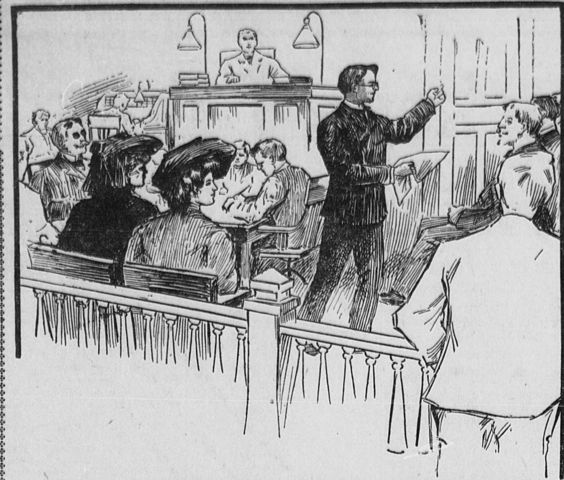
\includegraphics[scale=0.2]{figure/courtroom_sketch.jpg}
\end{frame}

%---------------------------------------------
\begin{frame}{$p$-value}
A \textbf{$p$-value} is the probability of obtaining a test statistic as extreme, or more extreme (in the direction of the alternative), than the observed value of the test statistic, assuming that $H_0$ is true.\\
\end{frame}

%---------------------------------------------
\begin{frame}{$p$-value}
Decision rule using the $p$-value:
\vspace{5pt}
\begin{itemize}
\item If $p$-value $< \alpha$, then reject $H_0$.
\item If $p$-value $> \alpha$, then do not reject $H_0$.
\end{itemize}
\vspace{10pt}
$\alpha$ is called the \textbf{signficance level}.\\  
Common values for $\alpha=0.05, 0.01$\\
\end{frame}

%---------------------------------------------
\begin{frame}{$p$-value}
\begin{itemize}
\item When the $p$-value $< \alpha$ (we reject $H_0$) the result is said to be \textbf{statistically significant}.
\vspace{10pt}
\item In other words, a result is statistically significant when it is unlikely to of occurred by random chance, assuming that the null hypothesis is true.
\vspace{10pt}
\item The smaller the $p$-value, the stronger the data favor $H_A$ over $H_0$.
\end{itemize}
\end{frame}

%---------------------------------------------
\begin{frame}
\begin{center}
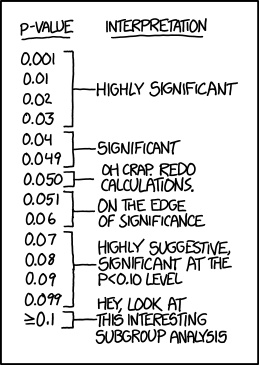
\includegraphics[scale=0.5]{figure/xkcd_p_values.png}
\end{center}

Image from \url{https://xkcd.com/1478/}
\end{frame}

%---------------------------------------------
\begin{frame}{Computing $p$-values}
\begin{columns}
\begin{column}{0.55\textwidth}
%\large
One-sided test (upper-tail):\\
$H_0: \mu = \mu_0$\\
$H_A: \mu > \mu_0$\\
\vspace{10pt}
Test statistic:\\
$$t = \frac{\bar{x} - \mu_0}{s/\sqrt{n}}$$\\
\vspace{10pt}

$p$-value $= \texttt{1 - pt(t, df = n-1)}$\\ 
\vspace{10pt}
Reject $H_0$ if $p$-value $< \alpha$\\
\end{column}
\begin{column}{0.45\textwidth}
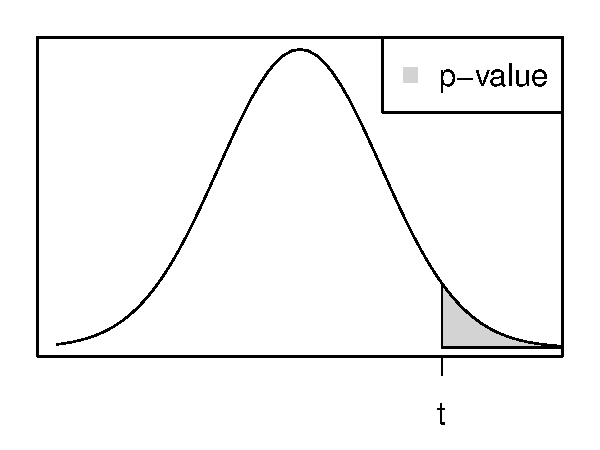
\includegraphics[scale=0.5]{figure/pvalue_upper.pdf}
\end{column}
\end{columns}
\vspace{1cm}
\end{frame}

%---------------------------------------------
\begin{frame}{Computing $p$-values}
\begin{columns}
\begin{column}{0.45\textwidth}
%\large
One-sided test (lower-tail):\\
$H_0: \mu = \mu_0$\\
$H_A: \mu < \mu_0$\\
\vspace{10pt}
Test statistic:\\
$$t = \frac{\bar{x} - \mu_0}{s/\sqrt{n}}$$\\
\vspace{10pt}

$p$-value $= \texttt{pt(t, df = n-1)}$\\ 
\vspace{10pt}
Reject $H_0$ if $p$-value $< \alpha$\\
\end{column}
\begin{column}{0.5\textwidth}
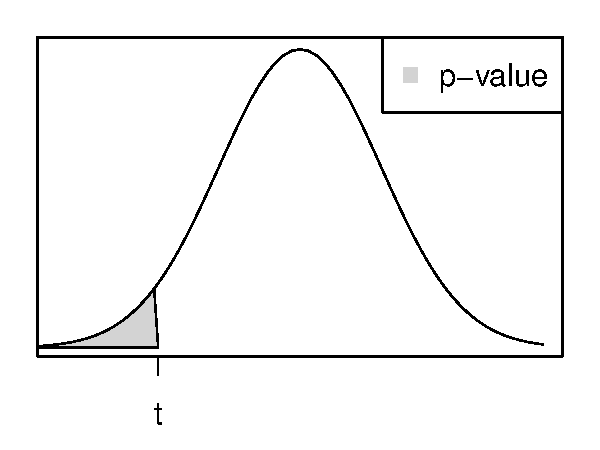
\includegraphics[scale=0.5]{figure/pvalue_lower.pdf}
\end{column}
\end{columns}
\vspace{1cm}
\end{frame}

%---------------------------------------------
\begin{frame}{Computing $p$-values}
\begin{columns}
\begin{column}{0.55\textwidth}
%\large
Two-sided test:\\
$H_0: \mu = \mu_0$\\
$H_A: \mu \neq \mu_0$\\
\vspace{10pt}
Test statistic:\\
$$t = \frac{\bar{x} - \mu_0}{s/\sqrt{n}}$$\\
\vspace{10pt}

$p$-value $= \texttt{2*pt(-abs(t), df = n-1)}$\\ 
\vspace{10pt}
Reject $H_0$ if $p$-value $< \alpha$\\
\end{column}
\begin{column}{0.45\textwidth}
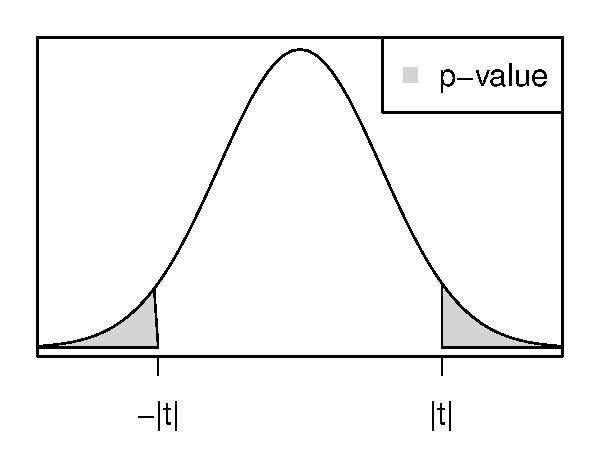
\includegraphics[scale=0.5]{figure/pvalue_both.pdf}
\end{column}
\end{columns}
\vspace{1cm}
\end{frame}

%---------------------------------------------
\begin{frame}{Conditions}
The hypothesis test is valid when the following conditions are satisfied:
\vspace{5pt}
\begin{itemize}
\item Sample observations are independent. Generally, this is satisfied when the data come from a random sample.
\item The sample size is large ($n \geq 30$), and there are no extreme outliers.  This implies that the sampling distribution for $\bar{X}$ is approximately normal according to the central limit theorem.
\item Otherwise, if the sample size is small ($n < 30$), the data should follow an approximate normal distribution. Graphical methods can be used to check this (box plot, histogram, normal QQ plot).\\
\end{itemize}
\vspace{3pt}
These are the same conditions that we need to check for a confidence interval for the population mean.\\

\bigskip
Note that when the sample size is large ($n \geq 30$) we can use either a $t$ or $z$ test statistic when computing the $p$-value (i.e., \texttt{pt()} and \texttt{pnorm()} will give approximately the same $p$-value).
\end{frame}

%---------------------------------------------
\begin{frame}{Example 1}
An administrator is interested in testing whether the average amount of time CSUEB students spend commuting to campus exceeds 1.5 hours.  A random sample of $n=20$ students are interviewed.  The sample mean $\bar{x} = 1.86$ and standard deviation $s=0.5$.  A histogram and QQ plot of the data are shown below.\\
\begin{figure}
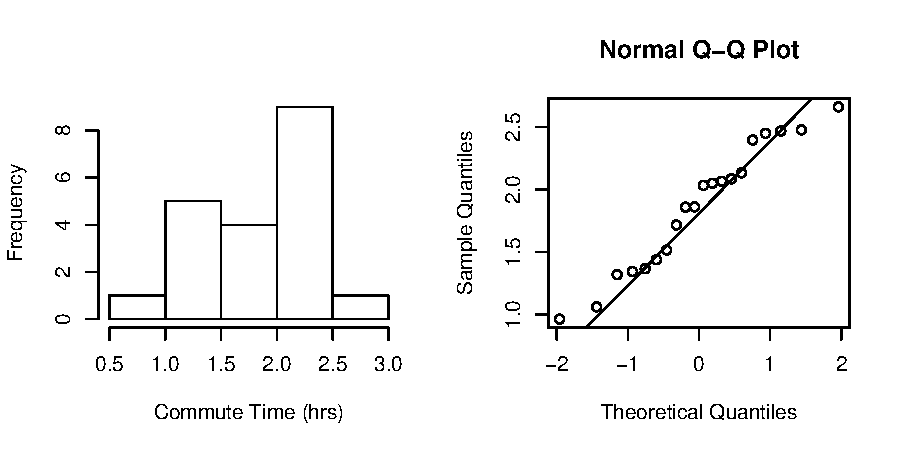
\includegraphics[scale=0.6]{figure/ex1.pdf}
\end{figure}
\end{frame}

%---------------------------------------------
\begin{frame}{Example 1}
\begin{enumerate}[(a)]
\item Write the null and alternative hypothesis for a one-sided test.
% \vspace{1cm}

\medskip
{\color{blue} $H_0: \mu = 1.5$\\
$H_A: \mu > 1.5$}
\smallskip

\item Check the conditions for the hypothesis test.
% \vspace{2.5cm}

\medskip
{\color{blue} The conditions for the test are satisfied:}\\
\begin{itemize}
{\color{blue}
\item Data come from a random sample
\item Data follow approximate normal distribution\\ 
(need to check since $n=20<30$)
}
\end{itemize}
\smallskip

\item Calculate the test statistic.
% \vspace{2.5cm}

{\color{blue}
$$t = \frac{\bar{x} - \mu_0}{s / \sqrt{n}} = 
\frac{1.86 - 1.5}{0.5 / \sqrt{20}} = 3.22$$
}
\end{enumerate}
\end{frame}

%---------------------------------------------
\begin{frame}{Example 1}
\begin{enumerate}[(a)]
\setcounter{enumi}{3}
\item Calculate the $p$-value and make a decision using $\alpha = 0.05$ significance level.

\smallskip
\begin{multicols}{2}
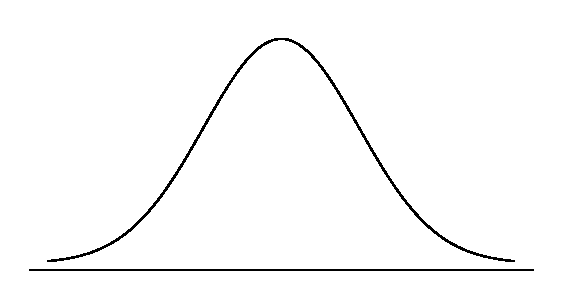
\includegraphics[scale=0.35]{figure/norm_draw.pdf}
\vspace{0.75cm}
\columnbreak

{\color{blue}$p$-value $= \texttt{1 - pt(3.22, df=19)} = 0.0023$\\
Since $p$-value $<0.05$, we reject $H_0$}
\end{multicols}


\item What is the conclusion of the test in the context of the data?
% \vspace{3.25cm}

\medskip
{\color{blue} The data provide strong evidence that the mean commute time for all CSUEB students is greater than 1.5 hours.}
\end{enumerate}
\end{frame}

%---------------------------------------------
\begin{frame}
\end{frame}

%---------------------------------------------
\begin{frame}{Example 2}
It is claimed that the mean mileage of a certain type of vehicle is 35 miles per gallon (mpg) of gasoline.  A random sample of 49 vehicles are collected.  The sample mean $\bar{x}=36.1$ mpg and standard deviation $s=5.4$ mpg. 
\begin{enumerate}[(a)]
\item Write the null and alternative hypothesis for a two-sided test.
% \vspace{1cm}

\medskip
{\color{blue} $H_0: \mu = 35$\\
$H_A: \mu \neq 35$}
\smallskip

\item Check the conditions for the hypothesis test.
% \vspace{2.5cm}

\medskip
{\color{blue} The conditions for the test are satisfied:}\\
\begin{itemize}
{\color{blue}
\item Data come from a random sample
\item Large sample size $n=49 > 30$
}
\end{itemize}

\end{enumerate}
\end{frame}

%---------------------------------------------
\begin{frame}{Example 2}
\begin{enumerate}[(a)]
\setcounter{enumi}{2}
\item Calculate the test statistic.
% \vspace{1.5cm}
{\color{blue}
$$t = \frac{\bar{x} - \mu_0}{s / \sqrt{n}} = 
\frac{36.1 - 35}{5.4 / \sqrt{49}} = 1.43$$}

\item Calculate the $p$-value and make a decision using $\alpha = 0.05$ significance level.

\smallskip
\begin{multicols}{2}
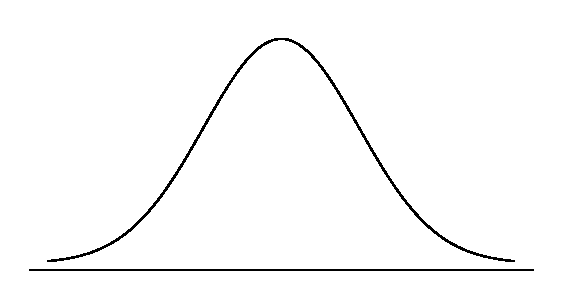
\includegraphics[scale=0.35]{figure/norm_draw.pdf}
\vspace{0.75cm}
\columnbreak

{\color{blue}
$p$-value $= \texttt{2*pt(-1.43, df=48)} = 0.159$\\
Since $p$-value $>0.05$, we do not reject $H_0$}
\end{multicols}

\item What is the conclusion of the test in the context of the data?
% \vspace{2cm}

\medskip
{\color{blue} The population mean mileage is \textbf{not} significantly different than 35 mpg.}
\end{enumerate}
\end{frame}

%---------------------------------------------
\begin{frame}{Decision Errors}
\begin{table}[ht]
\begin{tabular}{p{3cm}|p{3cm}|p{3cm}}
 &$H_0$ true  &  $H_A$ true \\
\hline
Reject $H_0$ \newline &  & \\
\hline
Do not reject $H_0$ \newline  &  &\\ 
\end{tabular}
\end{table}
% \vspace{3cm}

\bigskip
The significance level $\alpha$ is the probability of a type 1 error:
\begin{align*}
\alpha &= \text{Probability of rejecting $H_0$, when $H_0$ is true}\\
&= P(\text{reject } H_0 | H_0 \text{ true})
\end{align*}
\end{frame}

%---------------------------------------------
\begin{frame}{Decision Errors}
% \vspace{-3.5cm}
In a US court, the defendant is either innocent ($H_0$) or guilty ($H_A$).  What does a type 1 error represent in this context?  What does a type 2 error represent?\\
\bigskip

{\color{blue}
$H_0:$ The defendant is innocent\\
$H_A:$ The defendant is guilty\\
\bigskip

Type 1 error:\\ 
The defendant is actually innocent, but the jury decides guilty.\\
\medskip

Type 2 error:\\ 
The defendant is actually guilty, but the jury decides innocent.
}
\normalsize
\end{frame}

%---------------------------------------------
\begin{frame}{Using a confidence interval to perform a two-sided hypothesis test}

Suppose we want to perform the following two-sided test at the $\alpha$ level of significance:\\
\vspace{5pt}
$H_0: \mu = \mu_0$\\
$H_A: \mu \neq \mu_0$\\
\vspace{11pt}

Construct a $1-\alpha$ confidence interval (CI): 
\begin{align*}
\bar{x} \pm t_{\alpha/2; n-1} \frac{s}{\sqrt{n}}
\end{align*}
\begin{itemize}
\item If $\mu_0 \in \text{CI}$, then do not reject $H_0$
\item If $\mu_0 \not\in \text{CI}$, then reject $H_0$ in favor of $H_A$
\end{itemize}
\end{frame}

\begin{frame}{Example 3}
%\vspace{-3cm}
It is claimed that the mean mileage of a certain type of vehicle is 35 miles per gallon (mpg) of gasoline.  A random sample of 49 vehicles are collected. The sample mean $\bar{x}=36.1$ mpg and standard deviation $s=5.4$ mpg.  Use a confidence interval to perform the hypothesis test with $\alpha=0.05$.\\

\bigskip
\emph{Solution:}\\
$H_0: \mu = 35$; $H_A: \mu \neq 35$
$$\bar{x} \pm t_{\alpha / 2; n-1} \frac{s}{\sqrt{n}} \implies
36.1 \pm 2.01 \frac{5.4}{\sqrt{49}}
\implies (34.55, 37.65)$$
Since $\mu_0 = 35$ is inside the interval, we do not reject $H_0$ at the $\alpha = 0.05$ significance level.  We are 95\% confident that the population mean miles per gallon is between 34.55 and 37.65.
\end{frame}

\end{document}
